%!TEX root = ../main.tex
\setcounter{chapter}{7}
\setcounter{section}{2}
\section{Design using Discrete Equivalents}
\vspace{-8pt} \hrule \hrule \hrule \hrule \hrule  \vspace{12pt}
\begin{itemize}
\item (8.3.1) Tustin's Method
	\begin{enumerate}
		\item Tustin's method is a digitization technique that approaches the problem as one of numerical integration. Suppose 
		\begin{align*}
			\frac{U(s)}{E(s)}  = D_c(s) = \frac{1}{s} 
		\end{align*}
		which is integration. Therefore, it is corresponding to the \emph{trapezoidal integration} as follows:
		\begin{align*}
			u(kT) &= \int_{0}^{kT-T} e(t) dt + \int_{kT -T}^{kT} e(t) dt \\
			&= u(kT-T) + \mbox{area under $e(t)$ over last period, $T$},  \\
			&= u(kT-T) + T \frac{[e(kT-T)+e(kT)]}{2}\\
			u(k) &= u(k-1) + T \frac{[e(k-1)+e(k)]}{2}
		\end{align*}
		where $T$ is the sample period. 
		\begin{figure}[h] 
		    \centering
			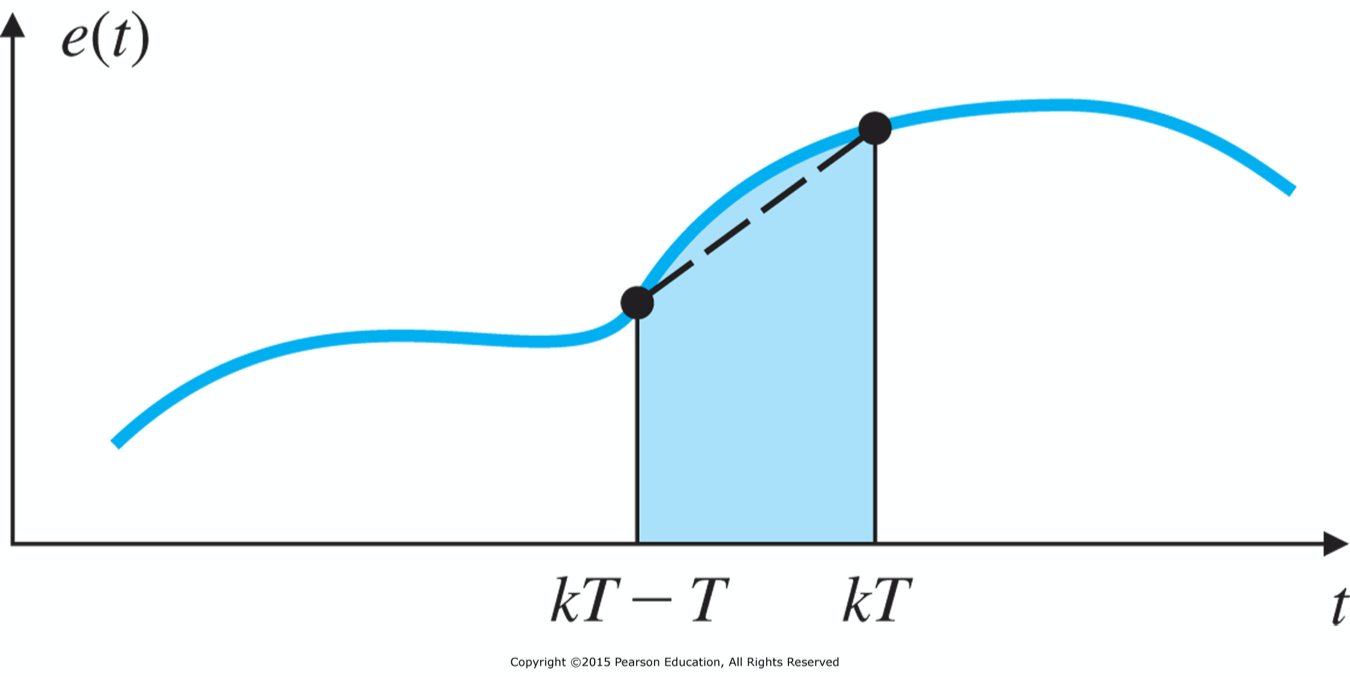
\includegraphics[width=8cm]{./FIG_Franklin/fig8-7.png}
		\end{figure}
		
	\end{enumerate}

\end{itemize}		